% This is a template for Ph.D. dissertations in the UCI format.

% All fonts, including those for sub- and superscripts, must be 10 points or larger.
% Recommended sizes are 14-point for chapter headings, 12-point for the main body of text
% and figure/table titles, and 10-point for footnotes, sub- and super-scripts, and text in
% figures and tables.
\documentclass[12pt,fleqn]{ucithesis}

\usepackage{amsmath}
\usepackage{array}
\usepackage{bm}
\usepackage{boxedminipage}
\usepackage{graphicx}
%\usepackage{natbib}
%http://merkel.zoneo.net/Latex/natbib.php
\usepackage[numbers]{natbib}
\usepackage{path}
\usepackage{psfrag}
\usepackage{relsize}
%\usepackage{subfigure}
\usepackage{subfig}
\usepackage{todonotes}
\usepackage{bytefield}
\usepackage{url}
\usepackage{verbatim}

% plainpages=false fixes the "duplicate ignored" error with page counters
% Set pdfborder to 0 0 0 to disable colored borders around PDF hyperlinks
\usepackage[plainpages=false,pdfborder={0 0 0}]{hyperref}



\graphicspath{{figures/}}

% Uncomment the following line to enable Unicode support. This will allow you
% to enter non-ASCII characters (such as accented characters) directly without
% having to use LaTeX's awkward escape syntax (e.g., \'{e})
% NOTE: You may have to install the ucs.sty package for this to work. See:
% http://www.unruh.de/DniQ/latex/unicode/
% \usepackage[utf8x]{inputenc}

\begin{document}


\thesistitle
{
  Improving the Architecture of Calico
}

\degreename{Master of Science}

% Use the wording given in the official list of degrees awarded by UCI:
% http://www.rgs.uci.edu/grad/academic/degrees_offered.htm
\degreefield{Informatics}

% Your name as it appears on official UCI records.
\authorname{Mitchell Ryan Dempsey}

% Use the full name of each committee member.
\committeechair{Professor Andr\'{e} van der Hoek}
\othercommitteemembers
{
  Professor James A. Jones\\
  Professor David F. Redmiles
}

\degreeyear{2012}

\copyrightdeclaration
{
  {\copyright} {\Degreeyear} \Authorname
}

% If you have previously published parts of your manuscript, you must list the
% copyright holders; see Section 3.2 of the UCI Thesis and Dissertation Manual.
% Otherwise, this section may be omitted.
% \prepublishedcopyrightdeclaration
% {
%   Chapter 4 {\copyright} 2003 Springer-Verlag \\
%   Portion of Chapter 5 {\copyright} 1999 John Wiley \& Sons, Inc. \\
%   All other materials {\copyright} {\Degreeyear} \Authorname
% }

% The dedication page is optional.
\dedications
{
  To my parents...
}

\acknowledgments
{
  I would like to thank...

  You must acknowledge grants and other funding assistance. 

  You may also acknowledge the contributions of professors and friends. 
  
  You also need to acknowledge any publishers of your previous work who have given you permission to incorporate that work into your dissertation. See Section 3.2 of the UCI Thesis and Dissertation Manual.
}


\thesisabstract
{
  The text of the abstract begins here. The text may contain a maximum of 350 words. Include a short statement of the problem you studied, a brief exposition of the methods and procedures employed in gathering the data, and a summary of your findings. No graphs, charts, or tables may be included.
}

\preliminarypages

\chapter{Introduction}

Software design tools offer the user a significant amount of power when it comes to tool support. 
Using these tools, designers can generate various design diagrams such as architecture diagrams, flowcharts, relational diagrams.
Tools have been created to support all forms of software design, ranging from object-oriented software design to database layouts to logic flow.
Many tools allow designers to create UML diagrams that can be used to represent a software program. ArgoUML \cite{argouml} is one such tool that has been downloaded thousands of times.
Other general tools such as Microsoft Visio \cite{visio} allow designers to create diagrams such as database layouts and flowcharts. 
Architectural diagram tools such as ArchStudio \cite{archstudio} allow designers to create a representation of a program's architecture and connections.
Many other tools exist; there is no shortage of tools to help designers create a broad range of different kinds of designs.


Despite these tools clearly helping in certain aspects of the design process, designers do not always use these tools.
When faced with a design problem, software designers will not necessarily use these tools from the start. 
As observed by Cherubini \cite{cherubini} and Petre \cite{petre}, many times designers will instead turn to a whiteboard or pen-and-paper in order to work through the design problem.


There are many reasons that designers turn to informal tools to help them during the design process. 
A few key benefits of using an informal design tool are listed below.
\begin{itemize}\itemsep1pt
\item 
Designers are free from the constraints of a formal design notation \cite{wong}. 
Using an informal design tool means that a designer is not required to create a formal design document. 
There is nothing to force them to adhere to UML, ERD, or any other formal notation. 
An informal tool allows the designer to easily sketch out a design in whatever notation works best for them. 
Designers want to work through a design quickly, without being bogged down by the details of the tool or the notation.
Formal design tools enforce strict adherence to a design notation.
When designers are forced to stop and create elements that adhere to the specific notation, they are wasting time that could be used to improve the design.

\item 
Sketching allows designers to keep up with their thinking process \cite{petre}. 
Designs can change at a fairly quick pace, and the tools that support designers need to be able to function effectively at this pace.
Formal design tools can be slow to create a design with, and this impedes the design process. 

\item 
Whiteboards and pen-and-paper are ideal mediums for collaboration.
They allow multiple designers to work at the same time on the same design.
Designs can be quickly created and modified by different designers at the same time, which helps improve the design process.
\end{itemize}

The affinity that designers have for using a whiteboard or pen-and-paper has been recognized across many different disciplines of design \cite{goel, cherubini}. 
Sketching plays a crucial and universal role in all fields of design. 
Despite this ubiquitous and advantageous role, a question arises whether sketching may be supported in a better way.
Using a whiteboard or pen-and-paper only allows a designer to add and delete content, nothing more.
What if there was software that was specifically designed to support the informal design process, rather than supporting the formal design process? 
What benefits would this software be able to provide designers?


This question is what led to the development of Calico \cite{calico2}. 
Calico is a software-sketching tool that aims to support designers by helping them easily draft potential software systems. 
Calico was designed to be used with a multi-touch whiteboard and projector so that it can replicate the role of a traditional whiteboard. 
The goal was to build upon the ease-of-use that a whiteboard provides designers, while at the same time providing options and benefits that a traditional whiteboard system lacks, such as the ability to revert to previous designs, or the ability to branch off designs. 
Calico has a number of features, such as ``scraps,'' gestures, and the grid, that were explicitly designed to support the informal design process.
Calico, is very similar to a traditional whiteboard in that it allows the user to sketch freely, but does not suffer from the disadvantages that a whiteboard does.


However, the early versions of Calico exhibited a number of problems when it came to supporting sketching and improving upon the traditional whiteboard experience tools.
\begin{itemize}\itemsep1pt
\item 
Distributed designers were not well supported.
The network system in Calico was sluggish, and as a result, distributed designers were not able to effectively collaborate with one another. The current network also did not function behind a firewall, so designers could only collaborate with designers on the local network.

\item 
Collaboration in early versions of Calico was not supported. 
Calico only supported a single user on a single ``canvas'', and designers were not able to work collaboratively on designs. 
As shown earlier, the ability to work collaboratively is one of the advantages of using a whiteboard or pen-and-paper, and without collaborative support, Calico was not equal to a whiteboard.

\item
It was very difficult to add new functionality, which prevented new features and plugins from being added. 

\end{itemize}
My research was about addressing these problems in order to improve Calico.


\chapter{Background}

To better understand our reasoning for creating Calico, it is useful to have some insight into the history of sketching, and in particular the history of sketching in software design. Designers rely on sketching as part of their own thought process.
% PD Stuff Here
When working collaboratively, designers use whiteboards to sketch design ideas, explore solutions, capture code fragments, decide on division of tasks as well as scheduling tasks. As discussed in\cite{chen1} the key advantages of using whiteboards for sketching include immediacy, versatility, size and collaboration. There is very little effort to access a whiteboard, whiteboards are capable of multiple as well as secondary mutations, the size allows for more than one sketch and finally a whiteboard allows multiple designers to work on and discuss evolving designs. 

Within the design literature several studies have looked at how designers behave when they are tasked with a complex design problem. Four general observations drove the development of Calico. Designers use low detail in sketching designs because the sketches are only initial thoughts and reflections\cite{a8} they are intentionally rought and without detail. Designers frequently shift their focus during intial phases and these original sketches are often revisited at a later time\cite{a9}. Designers often sketch, whether as a concious decision or not, ambiguous designs leaving room for later improvement\cite{a3}. Finally designers use a wide variety of languages when expressing designs whether it might be diagrams or informal symbols\cite{a6}. Calico was designed to aid software designers in creating and manipulating early software designs.
% /PD

Sketching allows designers to express their ideas in a very fluid and flexible manner.
Sketching allows designers to not be hindered by design software that tries to enforce a specific design style. Designers are able to be as meticulous as they wish, and they are not spending time working around the roadblocks created by a structured design system.
It is very easily for a designer to cross out a given idea and then immediately create an alternative. Designers typically work with a visual image in their head\cite{todo}, and sketching provides the least amount of friction when trying to put that visual image into the design.
This flexibility allows them to focus on the formation of ideas and discussion, without having to worry about how the discussion itself is being documented. 
Sketching allows ideas to be more easily viewed, analyzed, and discussed -- much more than would be possible without some representational notation.
Another benefit afforded by sketching is the ability to view a design from a higher-level or ``bird’s-eye view''.
This high-level view allows designers to discover design paths that they would have otherwise overlooked had the idea not been drawn out and understood. 

\todo{ANDRE: How is this unique to sketching versus a design tool?}
Sketching allows designers to create representations of concepts that can be linked together in order to create a very detailed design. For example, flowcharts can be created that show how logic will flow through a program. As another example, database designers can use sketching to informally show foreign key relations when designing a schema. 

Often in sketching, designers are able to mix very different design styles that a normal software design program would not be allow in the same space. As you can see in \todo{Add image}Figure, designers at a local company are creating sketches in order to design a software product. You can see how they have linked various components in the system to each other, so that they can create an overview of how the system will function.

% PD stuff here
The free flowing process of sketching allows for open-ended thought processes during initial phases of design, regardless of discipline. Sketching allows designers to have flexibility while they explore design problems. It allows them to go from abstract thoughts to concrete ideas\cite{todo}. Sketching allows designers to formulate new ideas, combine, transform, and also reject ideas\cite{todo}. In general, sketching allows the designer a path by which they can go from their original thoughts to a more concrete design. During this process, the designer can diverge from his original thoughts and gain insight from the sketching itself\cite{todo}.

Many have studied the value in sketching as the basis of the design process. Zannier found that tools that encouraged conversations between designers gave way to decisions that considered more alternatives\cite{todo}. Cherubini has found that designers use sketching as a way of brainstorming and manipulating concepts\cite{todo}. Software designers often sketch as a natural extension of the thought process used during the design phase to view more than a single solution simultaneously\cite{todo}.

\todo{ANDRE: Too fast, separate sections. 1) background of sketching 2) sketching tools}
Early tools, such as SILK\cite{todo} or DENIM\cite{todo} interpret shapes sketched by a user into model elements. Later tools such as SUMLOU\cite{todo} and Marama-Sketch\cite{todo} left the sketches in their original form until the user requested the translation into a formal diagram. Inkkit\cite{todo} advanced further by supporting multiple levels of formality. Other UML-oriented tools also followed similar design processes\cite{todo}.

While these programs do provide freedom of expression for a user, they still force the diagram into a specific notation. All of these tools focus on what can be sketched.

Early work in the computer-supported cooperative work (CSCW) community looked at how users can work collaboratively. Others have studied the interaction mechanisms and integrating tablet PC based input on a large display for a group of designers to work together\cite{todo}
% / PD


In the context of software design, sketching tools prove to be even more useful. These tools allow designers to create several varying solutions in parallel, and then chose the best of these designs to continue designing. Sketching allows software designers to fluidly move focus between various potential ideas in order to contrast designs with others. Software design tools that do not force a specific design structure on the user can encourage a broader consideration of alternative designs, and can greatly improve the eventual design outcome.

\chapter{Calico}

% [anticpated/actual features]
% [purpose, how does it work]
% [supports designers in sketching]

\section{Canvas and Grid}

\begin{figure}[htb]
\centering
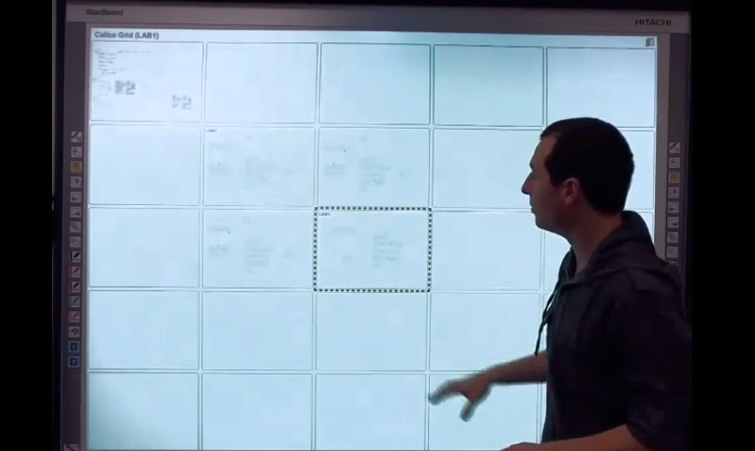
\includegraphics[width=0.8\textwidth]{grid.jpg}
\caption{The grid view within Calico}
\label{fig:grid}
\end{figure}
The grid is the focal point of any session in Calico.
It shows the various canvases that users may interact with in a given session.
Users may perform various operations on canvases from the grid, such as duplicating or clearing individual cells.
The grid also gives a clear overview of the designs that are happening in a session.

\section{Gestures}

\section{Scraps}
Scraps in Calico can be thought of as ``scraps of paper'' that one would place on a desk or on a white board.
Scraps can be easily relocated to different parts of the screen, or even other canvases.
Scraps can be stacked on top of each other and then treated as a unit or group.
By treating scraps as if they were pieces of paper, we [make it easy to understand the manipulation], as designers can easily relate Calico to their current design 

\section{Palette}
The palette in Calico provides users with a ``drawer'' that can easily be used to store commonly used shapes and artifacts.
The palette can be synchronized across sessions so that other users in the session can share the same palette.
\chapter{Objectives}

[old version was single user, list limitations] Calico was originally designed to be a single-user system that allowed individuals to operate an electronic whiteboard. While this original design worked great in an isolated environment, it made it very difficult for users to collaborate with one another. Users had to resort to taking screenshots and emailing them to one another.  Our aim with the new version of Calico was to create a system that would function in an isolated environment, but could easily facilitate collaboration with multiple users when needed. By designing with collaboration in mind, we were able to create a client-server architecture that would support many users interacting with the same canvas area simultaneously. The server had to be responsible for maintaining order of objects, as well as acting as a version control to make sure that users were not able to perform conflicting actions that would corrupt the drawings.

As an experiment, we worked to add collaboration to the original Calico implementation. This was able to help us determine that using Calico in a multi-user environment would be much more useful than we originally expected, and drove us to create a more robust multi-user implementation. Our attempts to [make old calico multi-user] were not successful, as the system was extremely sluggish and frustrated many users. We found that our users expected the system to be much more responsive, and the sluggishness was not acceptable. This was one of the biggest reasons that we decided to redesign a new Calico from the ground up.  

[reasoning for new iteration, rethinking architecture]Rather than continue working on the existing version of Calico, we discussed the [usefulness?] of redesigning the architecture from the ground up in order to better support the features we were hoping to add. We wanted to create a system based on the client-server architecture that would facilitate many clients all interacting with the system at the same time. The old version of Calico used a peer-to-peer connection that limited the number of active clients that could use the system. The old peer-to-peer architecture proved to be highly problematic when connecting with users over the Internet. While the system was able to work fine locally, the ultimate goal for the system was to collaborate with users all over the world, and we realized that a peer-to-peer architecture would not be ideal when collaborating over the Internet. This was one of the reasons we chose to move to a client-server architecture. We were able to place the server on a system that was open to the Internet, and it would eliminate all the connection problems that plagued the old peer-to-peer architecture. 

Another area where the client-server architecture benefitted us was with performance. We created a server that was highly optimized for processing data from many different clients at the same time. This allowed us to handle many more clients without any noticeable drop in processing time. Previous versions of Calico had the clients act as servers, which meant that in addition to processing all of the graphical data, they were also responsible for processing all incoming data and drawing what the other clients were sending.
[list requirements and wants/needs]
[req:distributed]
[req:persistence]The first iteration of Calico was a peer-to-peer system. This meant that there was no single place where the drawings would be stored. There was no way to view the contents of the session unless you were actively viewing it from within the Calico program itself. We wanted to be able to access the current state of a session without the need to actually join the session itself. By creating a central server that was responsible for maintaining the session, we were able to have a persistent history of the session. Users could join and disconnect, and then return, and still be able to undo operations that were performed long ago. Users could import canvas drawings into other programs by requesting a rendered image from the server. By storing the session state at a single location, we reduced the likelihood that data would become corrupted in transit, or data that would be corrupted synchronizing between many "master" servers as it had in the traditional peer-to-peer architecture. The persistent server was regarded as the true master, and if any client differed, it would synchronize with the central server, rather than assuming its own state was the "correct" version.

[req:sessions]Sessions was not initially planned in our rewrite of Calico, but we soon found a need for sessions to be added. The previous version of Calico had no session system at all, however it was not really necessary because users could essentially create their own sessions by just starting another instance of the program. This provided an easy method for users to work on various projects without interfering with the designs of another project. With the new client-server architecture, it was more difficult to start a new instance of the server in order to work on a separate project. Thus the need for sessions was realized, as designers needed a way to easily create a separate Calico instance that would not interfere with the existing session. 

[req:admin interface]One of the benefits of having a central server was the ability to have an "administrative interface" that could allow users to perform actions on the server, and backup/restore sessions. With the new version of Calico, we opted to create a web-based administrative interface that let the user perform various low-level commands that were used for debugging. Along with the ability to perform commands, users could download a file containing the entire state of a session. These files could then be restored at a later point in time, and would restore the session to its previous state. This proved to be very useful during the initial development, as it provided a safety net for users. Users were able to experiment more knowing they had a backup of their designs.

\chapter{High-Level Architecture}

Calico's new architecture was motivated by the design decisions listed below. 
The key design decisions for the new version of Calico were:

\begin{itemize}\itemsep1pt
  \item Client/Server architecture for improved connectivity over the Internet.
  \item Optimization of network traffic to reduce lag on distant clients, as well as network usage.
  \item A plugin framework to enable developers to create extensions into the Calico system.
  \item Improvement of input event handling system to improve drawing performance and input recognition.
  \item Consistency handling and persistence improvements to ensure that clients are all kept in the same state.
\end{itemize}

In the following sections, each decision will be explained in more detail.



\section{Client/Server Architecture}
We decided that the architecture needed to be redesigned in order to support all the planned changes. The new architecture that was chosen had to be able to support all the features, as well as easily support multiple users simultaneously. It also had to be accessible from anywhere, and had to be more stable than previous versions that were known to crash.

\begin{figure}[h]
\centering
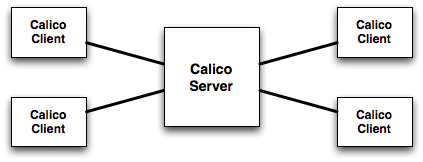
\includegraphics[width=0.8\textwidth]{arch_diag.png}
\caption{Overview of Calico's Architecture}
\label{fig:calico_arch}
\end{figure}

The first change made was a switch from the original peer-to-peer system to a completely new client-server architecture. We believed that by using a client-server architecture, we could provide a centrally accessible service that would easily support multiple clients and still maintain stability. The server could act as a headless service that could be more efficient since it did not have to perform any client functions such as rendering the display. This meant that the server could be dedicated to the task of managing all the interactions between clients, and could be much more stable than in a peer-to-peer context. When using peer-to-peer, each client was responsible for notifying all connected clients (which caused a large amount of network traffic). By switching to client-server, clients are only communicating with a single server, which greatly reduced the network traffic, and increased the stability of the network.

\section{Networking Component Overhaul}
One of the significant changes from the original Calico was the change in network communication design. The previous version of Calico had networking that was designed as an add-on at a later time, and was not fully integrated into the system. In this old design, when a change was made by another client, the entire change was saved to a Java object. This object was then serialized and sent in full over the network. The receiving client would deserialize this data, and then perform the change on its local drawing canvas. This process was very easy to implement, but had the cost of requiring significant processor time due to the constant serialization/deserialization process that would take place for each action. It also incurred the network overhead of Java serialization, which would add much more data to the final packet. All of this overhead would quickly become apparent to users when the system would lag in response to many actions done in quick succession. Our goal was to streamline this process as much as possible so that we could reduce lag when the system was being heavily utilized.

To improve the responsiveness of Calico, and reduce the network overhead, we created a custom packet design that could be used by Calico to notify both the client and server when various actions were performed. These special packets provided exactly what was needed to effectively communicate changes to clients, and thereby significantly reduced in size compared to the original design. Packets now are byte arrays that are written directly to the wire and, based on the format expected by the given command, are decoded back into their specific components (integers, strings, booleans, and floats). 



\begin{figure}[h!]
  \centering
  \begin{bytefield}{34}
    \bitbox{4}{length} & \bitbox{8}{command ID} & \bitbox{24}{command-specific data}
  \end{bytefield}
  \caption{A Calico network packet}
\label{fig:calico_packet}
\end{figure}

This packet design was loosely based on the packet design of the Half-Life game engine \cite{rcon}. As seen in the figure above, the packet is broken up into three main parts. The first four bytes of the packet is the length of the packet. This tells the network system how much farther it needs to read to ensure it receives the entire packet. The next four bytes hold the command identifier. This number is used to tell the network system what this packet is about. Both the client and the server have a list of commands and their IDs, which are used to translate from a programmer-friendly command name to the command ID number. The remaining bytes vary based on the specific command that is being transmitted. Each command has different parameters, of which both the client and server are aware. By writing data directly to the wire, there is little overhead -- each packet is as small as it could be. This makes the network communication between the client and server much more efficient, and helps to reduce the lag, even when put under heavy usage.

\section{Improvement of Input Handling System}
In the previous version of Calico, the input system was plagued by sluggish performance and inaccuracy. When there were many elements on the screen, the input system would lag and would begin to ``miss'' input data, which would result in straight lines instead of smooth curves. As a sketching tool, the ability to receive accurate input from the user was very important to the performance of the tool. The previous version of Calico routed input data directly to the rendering system, which would draw the images on screen. This made development very easy, but it required the input system to wait on the rendering process. This meant that the more images that had to be rendered, the longer the input system had to wait before it could start processing new input data. In Java, the mouse input listener does not queue input events -- if a program is too busy to receive input, then that input event is lost forever. Due to this problem, fluid drawing was nearly impossible.   

The new version of Calico is designed to fix this problem. By creating a separate, but dedicated input handling system, Calico can readily process input commands without having to wait for the rendering process to complete.

Instead of linking the input, action processing, and rendering systems serially, they are now linked in ``parallel'' using a multi-threaded approach. None of the separate processes are reliant on any of the other processes to complete, so input can be quickly received and queued if needed. These input events are then sent to the action processing system which determines what actions (if any) should be performed based upon the given input. Once an action is decided, the rendering process is notified and redraws the screen as needed. By using these components in parallel, we are able to remove the perceived lag and missed mouse events that would cause distortion and incorrect sketching. Even though the display can lag slightly behind the rendering system, this delay is not nearly as noticeable as when input events were being missed. 


\section{Consistency Handling / Persistence}
The previous version of Calico had many problems maintaining consistency between all clients. Clients would quickly become outdated and their states would not be consistent with that of the other clients. 
This problem was generally a result of parallel edits being performed. Clients would perform the edits locally, and then notify the other clients of the change. Often, the events would be received in a different order than they were being performed on a client, and the elements would be modified incorrectly. This led to identical elements being displayed very differently on multiple clients, due to the fact that there was no authority to resolve disputes when edits were being done to an element at the same time.
The previous version of Calico had no central server to check or update consistency, so any time where a client became inconsistent, designers had to quit the program and reconnect in order to fix the problem.
Naturally, this was very frustrating to users as it made it very difficult to collaborate with another user once the data became inconsistent. 

In the new version of Calico, this problem is fixed by implementing a system for checking and maintaining consistency across all clients connected to the server. In the new Calico, the server is considered to be the master, and all clients defer to the server to determine what state they should be at. All client actions are sent to the server and are not processed on the client until the server acknowledges the command. This means that all clients are given the same commands to modify elements at the same time. Clients are essentially ``unintelligent'' and do not assume any knowledge of where elements should be positioned -- this is all maintained by the server. This means that clients never become inconsistent, as there is a single system that is responsible for maintaining the state on each client system. 
Even when clients are editing the same element in parallel, Calico is able to maintain consistency by giving priority to the first event received. This allows users to edit the same element, and prevents the system from trying to issue conflicting edits to the same object.

The only time when clients now lose consistency was during network errors where packet loss is experienced. However, even if this were to occur, there are regular consistency checks that quickly realize the inconsistencies and fix them, without ever interrupting the designer. This system periodically notifies all clients of the current state of the system by sending a hash code to all clients. The hash code represents a checksum of the system and all of the drawing content. If any of the clients responds with a different hash code, they are sent an export of the entire session containing all the data needed to recreate the canvas from scratch. Because of this, any inconsistencies could easily be mitigated with minimal inconvenience to the end user. This meant that a session using the new version of Calico could last for weeks without problem -- something that was not possible in the previous version of Calico. The only drawback with this new process is that sometimes content changes unexpectedly for the user when parallel changes or packet loss occurs. While this is disruptive, the frequency of this occurring is low.

\chapter{Implementation}
Maybe talk about the actual technical implementation?
\chapter{Related Work}
%[what have other sketching tools done so far]
%[are there other distributed tools that do similar things]
%[what have we borrowed ideas from]

\chapter{Conclusion}
In conclusion, Calico is awesome.


% These commands fix an odd problem in which the bibliography line
% of the Table of Contents shows the wrong page number.
\clearpage
\phantomsection

% plain
%\bibliographystyle{abbrv} % DEFAULT
%\bibliographystyle{acm}
\bibliographystyle{abbrvnat}
\bibliography{thesis}

\appendix

\section{Calico Network Commands}
\begin{table}[h]
  \begin{tabular}{ | l | l | }
  \hline
  \textbf{Command Name} & \textbf{Format} \\ 
  \hline
  JOIN & SS \\
  \hline
  HEARTBEAT & LI \\
  \hline
  GROUP\_START & LLLI \\
  \hline
  GROUP\_APPEND & Lii \\
  \hline
  GROUP\_MOVE & LII \\
  \hline
  GROUP\_DELETE & L \\
  \hline
  GROUP\_DROP & L \\
  \hline
  GROUP\_FINISH & LB \\
  \hline
  GROUP\_SET\_CHILDREN & LII \\
  \hline
  GROUP\_SET\_PARENT & LL \\
  \hline
  GROUP\_MOVE\_START & L \\
  \hline
  GROUP\_MOVE\_END & LII \\
  \hline
  GROUP\_SET\_PERM & LI \\
  \hline
  GROUP\_RECTIFY & L \\
  \hline
  GROUP\_CIRCLIFY & L \\
  \hline
  GROUP\_CHILDREN\_COLOR & LIII \\
  \hline
  GROUP\_RELOAD\_START & LLLI \\
  \hline
  GROUP\_RELOAD\_FINISH & L \\
  \hline
  GROUP\_RELOAD\_COORDS & LIII \\
  \hline
  GROUP\_RELOAD\_CHILDREN & LIL \\
  \hline
  GROUP\_RELOAD\_POSITION & LII \\
  \hline
  GROUP\_RELOAD\_REMOVE & L \\
  \hline
  GROUP\_DUPLICATE & L \\
  \hline
  GROUP\_APPEND\_CLUSTER & LiII \\
  \hline
  GROUP\_SET\_CHILD\_GROUPS & Li \\
  \hline
  GROUP\_SET\_CHILD\_STROKES & Li \\
  \hline
  GROUP\_SET\_CHILD\_ARROWS & Li \\
  \hline
  GROUP\_REQUEST\_HASH\_CHECK & L \\
  \hline
  GROUP\_LOAD & LLLBiIIBddd \\
  \hline
  GROUP\_HASH\_CHECK & Li \\
  \hline
  GROUP\_COPY\_TO\_CANVAS & LLLII \\
  \hline
  GROUP\_SET\_TEXT & LS \\
  \hline
  GROUP\_SHRINK\_TO\_CONTENTS & L \\
  \hline
  GROUP\_IMAGE\_DOWNLOAD & LLSII \\
  \hline
  GROUP\_IMAGE\_LOAD & LLLSIIIIBiII \\
  \hline
  GROUP\_ROTATE & Ld \\
  \hline
  GROUP\_SCALE & Ldd \\
  \hline
  GROUP\_CREATE\_TEXT\_GROUP & LLSII \\
  \hline
  GROUP\_MAKE\_RECTANGLE & LIIII \\
  \hline
  GRID\_SIZE & II \\
  \hline
  UUID\_BLOCK & ILL \\
  \hline
  \end{tabular}
\end{table}

\begin{table}[h]
  \begin{tabular}{ | l | l | }
  \hline
  \textbf{Command Name} & \textbf{Format} \\ 
  \hline
  CANVAS\_INFO & LSII \\
  \hline
  CANVAS\_UPDATE & L \\
  \hline
  CANVAS\_UNDO & L \\
  \hline
  CANVAS\_REDO & L \\
  \hline
  CANVAS\_RELOAD\_START & L \\
  \hline
  CANVAS\_RELOAD\_FINISH & L \\
  \hline
  CANVAS\_RELOAD\_STROKES & LIL \\
  \hline
  CANVAS\_RELOAD\_GROUPS & LIL \\
  \hline
  CANVAS\_RELOAD\_ARROWS & LIL \\
  \hline
  CANVAS\_CLEAR\_FOR\_SC & L \\
  \hline
  CANVAS\_SC\_FINISH & L \\
  \hline
  CANVAS\_LOCK & LBSL \\
  \hline
  STATUS\_MESSAGE & S \\
  \hline
  ERROR\_MESSAGE & S \\
  \hline
  ERROR\_POPUP & S \\
  \hline
  CLICK\_TRACK & I \\
  \hline
  BGE\_APPEND & LII \\
  \hline
  BGE\_COLOR & LIII \\
  \hline
  BGE\_COORDS & LIII \\
  \hline
  BGE\_DELETE & L \\
  \hline
  BGE\_FINISH & L \\
  \hline
  BGE\_MOVE & LII \\
  \hline
  BGE\_START & LLL \\
  \hline
  BGE\_PARENT & LL \\
  \hline
  BGE\_CONSISTENCY & L \\
  \hline
  BGE\_RELOAD\_START & LLLIII \\
  \hline
  BGE\_RELOAD\_COORDS & LIII \\
  \hline
  BGE\_RELOAD\_FINISH & L \\
  \hline
  \end{tabular}
\end{table}

\begin{table}[h]
  \begin{tabular}{ | l | l | }
  \hline
  \textbf{Command Name} & \textbf{Format} \\ 
  \hline
  STROKE\_RELOAD\_START & LLLIII \\
  \hline
  STROKE\_RELOAD\_COORDS & LIII \\
  \hline
  STROKE\_RELOAD\_FINISH & L \\
  \hline
  STROKE\_RELOAD\_REMOVE & L \\
  \hline
  STROKE\_RELOAD\_POSITION & LII \\
  \hline

  STROKE\_START & LLLIII \\
  \hline
  STROKE\_APPEND & LiII \\
  \hline
  STROKE\_FINISH & L \\
  \hline
  STROKE\_SET\_COLOR & LIII \\
  \hline
  STROKE\_SET\_PARENT & LL \\
  \hline
  STROKE\_MOVE & LII \\
  \hline
  STROKE\_DELETE & L \\
  \hline
  STROKE\_LOAD & LLLCidddII \\
  \hline
  STROKE\_HASH\_CHECK & L \\
  \hline
  STROKE\_MAKE\_SCRAP & LL \\
  \hline
  STROKE\_MAKE\_SHRUNK\_SCRAP & LL \\
  \hline
  STROKE\_DELETE\_AREA & LL \\
  \hline
  STROKE\_ROTATE & Ld \\
  \hline
  STROKE\_SCALE & Ldd \\
  \hline
  STROKE\_SET\_AS\_POINTER & L \\
  \hline
  STROKE\_HIDE & LB \\
  \hline
  STROKE\_UNHIDE & L \\
  \hline

  ERASE\_START & L \\
  \hline
  ERASE\_END & LB \\
  \hline

  PLUGIN\_EVENT & S \\
  \hline



  CONSISTENCY\_CHECK &  \\
  \hline
  CONSISTENCY\_FINISH &  \\
  \hline
  CONSISTENCY\_CHECK\_CONTINUE & L \\
  \hline
  CONSISTENCY\_FAILED &  \\
  \hline
  CONSISTENCY\_RESYNC\_CANVAS & L \\
  \hline


  ARROW\_CREATE & LLICILIIILII \\
  \hline
  ARROW\_DELETE & L \\
  \hline
  ARROW\_SET\_TYPE & LI \\
  \hline
  ARROW\_SET\_COLOR & LIII \\
  \hline


  BACKUP\_FILE\_INFO & L \\
  \hline
  BACKUP\_FILE\_START &  \\
  \hline
  BACKUP\_FILE\_END &  \\
  \hline
  BACKUP\_FILE\_ATTR & SS \\
  \hline

  LIST\_CREATE & LLLLI \\
  \hline
  LIST\_LOAD & LLLBiII \\
  \hline
  LIST\_CHECK\_SET & LLLLB \\
  \hline
  \end{tabular}
\end{table}

Formats:
S-string. s-short. C-color. c-char. L-long. I-signed integer. i-unsigned integer. B-boolean. b-byte. f-float. d-double

%\section{Appendix A}

\end{document}
